% Nama Kelompok : Kelompok 3
% Kelas : D4 TI 1A
% 1. Kadek Diva Krishna Murti (1174006)
% 2. Niko
% 3. Rizal Rony Sitorus
% 4. Jeremia
% 5. Sri Rahayu (1174015)

\section{Pengertian Bit Parity}
Bit Parity merupakan bit tambahan yang disisipkan pada urutan bit-bit data yang ditransmisikan.
Tujuan pemberian bit parity ini adalah untuk memastikan bahwa bit - bit yang ditransmisikan tidak mengalami perubahan nilai setelah sampai di penerima.
Perubahan nilai dapat terjadi karena pengaruh noise atau sinyal liar.
Perubahan nilai : 0 $\,\to\,$ 1 atau 1 $\,\to\,$ 0
\newline Contoh :

\begin{table}[h!]
\centering
\begin{tabular}{ c c c }
0110100 & $\,\to\,$ &  0100100\\
\hline
Tx &  & Rx \\
\end{tabular}
\end{table}

\begin{figure}[ht]
\centerline{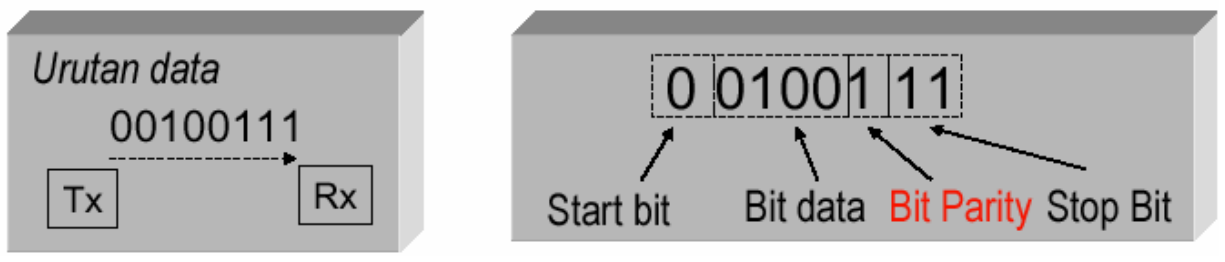
\includegraphics[width=1\textwidth]{figures/perubahan_nilai_bit_parity.png}}
\caption{Contoh perubahan nilai pada bit parity.}
\label{perubahan_nilai_bit_parity}
\end{figure}

Proses perubahan nilainya bisa dilihat pada gambar \ref{perubahan_nilai_bit_parity}

\section{Cara Kerja Bit Parity}
\subsection{Konsep Umum}
Pihak pengirim akan menambahkan 1 bit tambahan (Bit Parity) pada data, untuk menggabarkan karakteristik dari data tersebut. Nilai dari bit parity (1 atau 0) tidak diperbolehkan secara sembarang. Dalam proses pentransmisiannya data tadi dikirim bersamaan (data dan bit parity-nya). Pada terminal penerimaan data kita dibaca dan di dekodisasi dengan cara yang sama seperti saat menentukan nilai bit parity disisi pengirim. Lalu hasil dekodisasi tadi dibandingkan dengan bit parity yang dibawakan oleh pengirim.
Apabila hasil pembacaan (dekodisasi) data terkirim sama dengan bit Paritynya maka data tersebut dapat dianggap benar. Dan apabila diperoleh perbedaan nilai antara hasil dekodisasi dengan bit Paritynya maka data dapat di klasifikasi sebagai data yang error. Terminal penerima akan mengirim request pada terminal pengirim untuk mengirim ulang data yang error.
 
\subsection{Menentukan Nilai Bit Parity}
Penentuan nilai bit Parity (1 atau 0) dilakukan dengan meng-XOR kan semua bit yang ada pada data sepasang-sepasang, hasil akhir dari peng-XOR an seluruh bit ini yang akan dijadikan acuan untuk menentukan nilai dari bit Parity yang akan ditambahkan. Jadi belum tentu hasil XOR langsung dijadikan sebagai nilai dari bit Parity.


%%%%%%%%%%%%%%%%%%%%%%%%%%%%%%%%%% KADEK DIVA KRISHNA MURTI %%%%%%%%%%%%%%%%%%%%%%%%%%%%%%%%%%%%%

\section{Kelebihan dan Kekurangan Bit Parity}
\subsection{Kelebihan Bit Parity}
-   Lebih cepat karena berbasis 2 (biner)
-   Mudah dalam pengecekan
-   Sederhana dalam analisis dan penggunaan pada sistem
-   Mudah direalisasikan dalam bentuk rangkaian atau hardware

\subsection{Kekurangan Bit Parity}
-   Kurang handal dalam mengatasi deteksi dan perbaikan error
-   Kemungkinan kesalan yang terjadi besar, yaitu 50%
-   Belum dapat mengakomodir file dengan ukuran besar
-   Tidak dapat mendeteksi kesalahan dalam jumlah genap

%%%%%%%%%%%%%%%%%%%%%%%%%%%%%%%% NICO EKKLESIA SEMBIRING %%%%%%%%%%%%%%%%%%%%%%%%%%%%%%%%%%%%%%%


